\documentclass{article}

\usepackage[left=2cm,right=2cm, top=2cm, bottom = 2cm]{geometry}
\usepackage{amsfonts}
\usepackage{amsmath}
%%%\usepackage{array}

\usepackage{tikz}

\pagestyle{empty}

\setlength{\tabcolsep}{15pt}
%%%\renewcommand{\arraystretch}{2.5}

%%%\makeatletter
%%%\newcommand{\thickhline}{%
%%%    \noalign {\ifnum 0=`}\fi \hrule height 2pt
%%%    \futurelet \reserved@a \@xhline
%%%}
%%%\newcolumntype{!}{@{\hskip\tabcolsep\vrule width 2pt\hskip\tabcolsep}}
%%%\makeatother

\def\ihat{\hat{\i}}
\def\jhat{\hat{\j}}

\begin{document}

\title{Rotations and Compound Angle Formulae}
\date{}

\maketitle
\thispagestyle{empty}

\Large

\textbf{\underline{Objective: To understand the effect of a rotation on the coordinates}}

\textbf{\underline{of a point, and be able to use the compound angle formulae for}}

\textbf{\underline{trigonometric functions}}



\vspace{5mm}


\textbf{Recap of previous material:}

\vspace{5mm}


\begin{enumerate}
\item Sketch the graph of $y=x^3$. Hence sketch the graph of $y=(2x-3)^3-1$.
\item Identify the amplitude, angular frequency, ordinary frequency, and phase of the sinusoid $7\sin(\pi t-1.42)$. Sketch its graph.
\item Identify the amplitude, angular frequency, ordinary frequency, and phase of the sinusoid $-3\cos(2(t-1))$. Sketch its graph. Be careful---this one is tricky!
\end{enumerate}


\clearpage


\textbf{Warm-up:}

\vspace{5mm}

Let's explore rotations of points about the origin.

\begin{enumerate}
\item Suppose the point $(1,0)$ is rotated anticlockwise by an angle $\theta$. What are its new coordinates? Hint: think about the definition of sin and cos.
\item Suppose the point $(0,1)$ is rotated anticlockwise by an angle $\theta$. What are its new coordinates? Hint: compare with $(1,0)$.
\item Suppose the points $(1,0)$, $(0,1)$, and $(a,b)$ are rotated anticlockwise by $\frac{\pi}{2}$.
	\begin{enumerate}
	\item What are the coordinates of the rotations of $(1,0)$ and $(0,1)$?
	\item The rotated coordinates of $(a,b)$ are $(-b,a)$.
	We can relate the original coordinates to each other by the equation
	\[ (a,b) = a(1,0) + b(0,1).\]
	Write a similar equation linking the coordinates of the rotated points.
	\end{enumerate}
\item Suppose the points $(1,0)$, $(0,1)$, and $(a,b)$ are rotated anticlockwise by $\frac{3\pi}{4}$.
	\begin{enumerate}
	\item What are the coordinates of the rotations of $(1,0)$ and $(0,1)$?
	\item The rotated coordinates of $(a,b)$ are
	\[\left(\frac{-a}{\sqrt{2}}-\frac{b}{\sqrt{2}},\frac{b}{\sqrt{2}}-\frac{a}{\sqrt{2}}\right).\]
	We can relate the original coordinates to each other by the equation
	\[ (a,b) = a(1,0) + b(0,1).\]
	Write a similar equation linking the coordinates of the rotated points.
	\end{enumerate}
\end{enumerate}




\clearpage

\textbf{Theory---Vectors and Rotations:}

\vspace{5mm}

Think of the point $(1,0)$ as instructions ``go one unit to the right.'' Call this instruction $\ihat$. Similarly, $(0,1)$ is the instruction ``go one unit upwards.'' Call this $\jhat$. Then a general point $(a,b)$ may be thought of as $a\ihat+b\jhat$---``go $a$ to the right and $b$ upwards.'' We call $\ihat$ and $\jhat$ the \textbf{standard unit vectors}.

\begin{center}
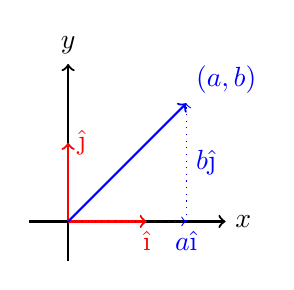
\begin{tikzpicture}
\draw[thick,->] (-0.5,0) -- (2,0);
\node[right] at (2,0) {$x$};
\draw[thick,->] (0,-0.5) -- (0,2);
\node[above] at (0,2) {$y$};

\draw[red,thick,->] (0,0) -- (1,0);
\node[below,red] at (1,0) {$\ihat$};
\draw[red,thick,->] (0,0) -- (0,1);
\node[right,red] at (0,1) {$\jhat$};

\draw[blue,thick,->] (0,0) -- (1.5,1.5);
\node[blue, above right] at (1.5,1.5) {$(a,b)$};
\draw[dotted,blue,->] (0,0) -- (1.5,0);
\node[blue, below] at (1.5,0) {$a\ihat$};
\draw[dotted,blue,->] (1.5,0) -- (1.5,1.5);
\node[blue,right] at (1.5,0.75) {$b\jhat$};
\end{tikzpicture}
\end{center}

Let $R$ denote rotation by an angle $\theta$. Then $R(\ihat)$ is the instruction ``move one unit in the direction $\theta$ above the positive $x$-axis'' and $R(\jhat)$ is the instruction ``move one unit in the direction $\theta$ anticlockwise of the positive $y$-axis.'' Rotate the whole setup above by $\theta$:

\begin{center}
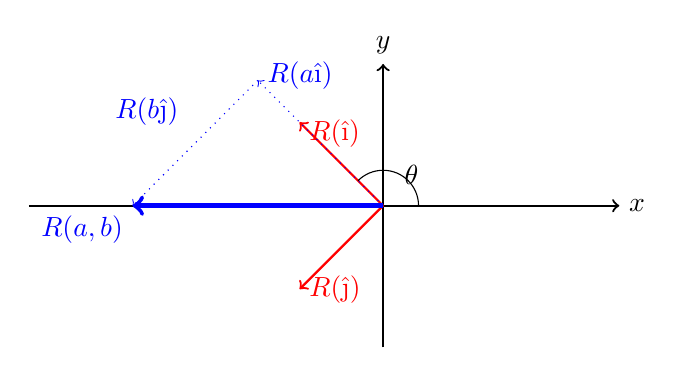
\begin{tikzpicture}[scale=1.5]
\draw[thick,->] (-3,0) -- (2,0);
\node[right] at (2,0) {$x$};
\draw[thick,->] (0,-1.2) -- (0,1.2);
\node[above] at (0,1.2) {$y$};

\draw[red,thick,->] (0,0) -- (-0.707,0.707);
\node[right,red] at (-0.707,0.607) {$R(\ihat)$};
\draw[red,thick,->] (0,0) -- (-0.707,-0.707);
\node[right,red] at (-0.707,-0.707) {$R(\jhat)$};
\draw (0.3,0) arc (0:135:0.3);
\node[above right] at (0.1,0.1) {$\theta$};

\draw[blue,ultra thick,->] (0,0) -- (-2.121,0);
\node[blue, below left] at (-2.121,0) {$R(a,b)$};
\draw[dotted,blue,->] (0,0) -- (-1.061,1.061);
\node[blue, right] at (-1.061,1.1) {$R(a\ihat)$};
\draw[dotted,blue,->] (-1.061,1.061) -- (-2.121,0);
\node[blue] at (-2,0.8) {$R(b\jhat)$};
\end{tikzpicture}
\end{center}

Rotating everything by $\theta$ doesn't affect the \textit{relative angles}. So if $R$ is any rotation, we have
\[R(a\ihat+b\jhat)=aR(\ihat)+bR(\jhat).\]

So to understand a rotation, it is enough to understand what it does to the \textbf{unit vectors} $\ihat$ and $\jhat$. We saw in the warm-up that, for rotation by angle $\theta$:
\[R(\ihat) = (\cos(\theta),\sin(\theta))=\cos(\theta)\ihat+\sin(\theta)\jhat\]
\[R(\jhat)=(-\sin(\theta),\cos(\theta))=-\sin(\theta)\ihat+\cos(\theta)\jhat.\]

Therefore we have:
\begin{align*}
R(a,b) &=aR(\ihat)+bR(\jhat)\\
&= a(\cos(\theta)\ihat+\sin(\theta)\jhat)+b(-\sin(\theta)\ihat+\cos(\theta)\jhat)\\
&= (a\cos(\theta)-b\sin(\theta))\ihat+(a\sin(\theta)+b\cos(\theta))\jhat\\
&=\left(a\cos(\theta)-b\sin(\theta),\; a\sin(\theta)+b\cos(\theta)\right)
\end{align*}



\clearpage


\textbf{Practice:}

\vspace{5mm}

Recall: The formula derived above is that if the point $(a,b)$ is rotated by an angle $\theta$, its new coordinates are:
\[\left(a\cos(\theta)-b\sin(\theta),\; a\sin(\theta)+b\cos(\theta)\right).\]

\begin{enumerate}
\item Find the new coordinates of the point $(7,2)$ after a rotation by $\frac{\pi}{3}$.
\item Find the new coordinates of the point $(-4,3)$ after a rotation by $-1.97$.
\item A point is rotated by an angle $\frac{\pi}{12}$, after which its coordinates are $(1.6,-2.9)$. What were the original coordinates of the point? Hint: think how geometrically to undo a rotation.
\end{enumerate}

\clearpage


\textbf{Application---Compound Angle Formulae:}

\vspace{5mm}

We shall use rotations to derive the \textbf{compound angle formulae}. These are important trigonometric identities relating trig functions of two angles $\alpha$ and $\beta$ with trig functions of their sum $\alpha+\beta$. The idea we will follow is to form an angle $\alpha+\beta$ by starting at an angle $\alpha$ and rotating by $\beta$; by doing this in both polar and cartesian coordinates, we shall obtain the compound angle formulae.

Recall: The formula derived above is that if the point $(a,b)$ (in cartesian coordinates) is rotated by an angle $\theta$, its new coordinates are:
\[\left(a\cos(\theta)-b\sin(\theta),\; a\sin(\theta)+b\cos(\theta)\right).\]

\begin{enumerate}
\item What are the cartesian coordinates of the point $P$ whose polar coordinates are $(1,\alpha)$?
\item In polar coordinates, the formula for a rotation is much easier than in cartesian coordinates. Write down the polar coordinates of the point obtained by rotating $P$ through an angle $\beta$. Call this rotated point $R(P)$.
\item Express $R(P)$ in cartesian coordinates.
\item By comparing your answer to question 3 with the cartesian rotation formula above, derive the following \textbf{compound angle formulae}:
\[\cos(\alpha+\beta)=\cos(\alpha)\cos(\beta)-\sin(\alpha)\sin(\beta),\]
\[\sin(\alpha+\beta)=\sin(\alpha)\cos(\beta)+\cos(\alpha)\sin(\beta).\]
\item Hence deduce the compound angle formula for tan:
\[\tan(\alpha+\beta) = \frac{\tan(\alpha)+\tan(\beta)}{1-\tan(\alpha)\tan(\beta)}.\]
\end{enumerate}



\clearpage


\textbf{Key Points to Remember:}

\begin{enumerate}
\item The \textbf{standard unit vectors} are $\ihat=(1,0)$ and $\jhat=(0,1)$, thought of as instructions to move one unit to the right or upwards, respectively.
\item Any point with cartesian coordinates $(a,b)$ can be expressed in terms of the standard unit vectors as $a\ihat+b\jhat$.
\item Applying a rotation $R$ does not affect the \textit{relative} positions of the vectors, so $R(a,b)=aR(\ihat)+bR(\jhat)$. So a rotation is \textit{completely determined} by what it does to the standard unit vectors.
\item In \textbf{cartesian coordinates}, rotation by angle $\theta$ moves the point $(a,b)$ to
\[\left(a\cos(\theta)-b\sin(\theta),\; a\sin(\theta)+b\cos(\theta)\right).\]
\item In \textbf{polar coordinates}, rotation by angle $\phi$ moves the point $(r,\theta)$ to $(r,\theta+\phi)$.
\item The \textbf{compound angle formulae} are:
	\[\cos(\alpha+\beta)=\cos(\alpha)\cos(\beta)-\sin(\alpha)\sin(\beta),\]
	\[\sin(\alpha+\beta)=\sin(\alpha)\cos(\beta)+\cos(\alpha)\sin(\beta).\]
	\[\tan(\alpha+\beta) = \frac{\tan(\alpha)+\tan(\beta)}{1-\tan(\alpha)\tan(\beta)}.\]
\end{enumerate}




\end{document}